\section{Introduction}


\begin{frame}{The Present Cipher}
\begin{itemize}
    \item Ultra-Lightweight block cipher.
    \item Developed by the Orange Labs (France), Ruhr University Bochum (Germany) and the Technical University of Denmark in 2007.
    \item Supports 64 bits block size and 80 or 128 bits key sizes with 31 rounds.
    \item Intended to be used in circumstances where high chip performance and low power consumption are required. 
\end{itemize}
\end{frame}

\begin{frame}{Substitution/ Permutation}
\begin{figure}[H]
    \centering
    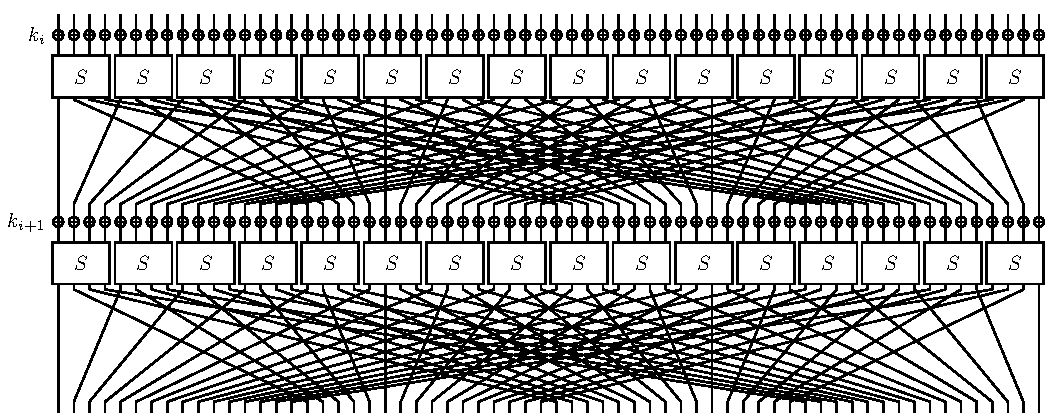
\includegraphics[width=\linewidth]{PRESENT_diagram.pdf}
\end{figure}
\begin{center}
    \scalebox{0.95}{
    \begin{tabular}{ |c||c|c|c|c|c|c|c|c|c|c|c|c|c|c|c|c| }
        \hline
        $x$ & 0 & 1 & 2 & 3&4& 5& 6&7&8&9&A&B&C&D&E&F  \\ \hline
        $S[x]$& C & 5 & 6& B &9 &0 &A &D& 3& E &F& 8& 4 &7& 1& 2 \\ \hline
    \end{tabular}}\\
    Image source : iacr.org/authors/tikz/
\end{center}
\end{frame}